\chapter{Implementation and Testing Results}\label{ch:implementation-and-testing-results}
\justify

The implementation phase of the project has followed a systematic approach, incorporating all the steps and methods mentioned in the previous chapters.
This phase has utilized the mentioned tools and technologies to achieve the project's objectives effectively and efficiently.

\section{OSINT Data Mining Software}\label{sec:osint-data-mining-software}
\begin{enumerate}[label=\roman*.]
    \item \textbf{Frontend:}
    \begin{itemize}
        \item .NET Framework: Proprietary framework by Microsoft, primarily for Windows.
        \item WhatsApp Chatbot: Integrated for user interaction.
    \end{itemize}

    \item \textbf{Backend:}
    \begin{itemize}
        \item Express.js: Integrated with various technologies.
        \begin{enumerate}[label=\arabic*.]
            \item \textbf{Court Checker:} Third-party tool with a large collection of Indian court cases, updated daily.
            \item \textbf{OSINT Search:} Gathers publicly available information to aid investigations.
            \item \textbf{Vehicle Information:} Retrieves details of vehicles using registration numbers.
        \end{enumerate}
    \end{itemize}

    \item \textbf{Database:}
    \begin{itemize}
        \item Data collected from external APIs.
        \begin{enumerate}[label=\arabic*.]
            \item \textbf{Court Checker:} Third-party tool with a large collection of Indian court cases, updated daily.
            \item \textbf{OSINT Search:} Gathers publicly available information to aid investigations.
            \item \textbf{Vehicle Information:} Retrieves details of vehicles using registration numbers.
        \end{enumerate}
        \item Data collected from scraping users' data from the internet.
        \begin{enumerate}[label=\arabic*.]
            \item \textbf{Facebook:} Scraping Facebook profile names, photos, emails, and cities with Puppeteer using a username.
            \item \textbf{WhatsApp:} Collecting WhatsApp user images, names, about, and online status.
            \item \textbf{Leak OSINT:} Scraping users' leaked data from the internet.
        \end{enumerate}
        \item Data collected from Call One App.
        \begin{enumerate}[label=\arabic*.]
            \item \textbf{Contacts:} The app collects users' contacts when the user first registers to the app and when a new contact is created.
            \item \textbf{Call Logs:} The app collects users' call logs every day and resolves the names of unknown calls.
            \item \textbf{Location Information:} User location is captured by the app as per the security requirements.
            The shared location is used for law enforcement purposes to track users' locations by the police department.
        \end{enumerate}
    \end{itemize}
\end{enumerate}

\subsection{Call One Old Architecture}\label{subsec:old-architecture}

The old architecture was built on React Native, but the app was very slow due to the bridge in React Native.
\begin{enumerate}[label=\roman*.]
    \item \textbf{Frontend:}
    \begin{itemize}
        \item React Native: Intuitive UI for data collection and settings.
    \end{itemize}

    \item \textbf{Backend:}
    \begin{itemize}
        \item Express.js: Integrated with various technologies.
        \begin{enumerate}[label=\arabic*.]
            \item \textbf{Express.js:} Minimal and flexible Node.js web application framework.
            \item \textbf{PostgreSQL:} Stores user details like contacts, call logs, and device information.
            \item \textbf{Crypto-js:} Uses AES Encryption to encrypt user information transmitted over the server.
        \end{enumerate}
    \end{itemize}
\end{enumerate}

\subsection{Call One New Architecture}\label{subsec:new-architecture}
In the new architecture, Kotlin was used along with additional services and optimizations.
\begin{enumerate}[label=\roman*.]
    \item \textbf{Frontend:}
    \begin{itemize}
        \item Kotlin: Used to develop the app with Jetpack Compose for UI\@.
    \end{itemize}

    \item \textbf{Backend:}
    \begin{itemize}
        \item Same as old architecture.
    \end{itemize}
\end{enumerate}

\subsection{New Features in Call One}\label{subsec:new-features}
The new architecture introduced several new features:
\begin{itemize}
    \item \textbf{Appication Speed:} App speed is increased by using kotlin.
    \item \textbf{New UI:} A new Material UI is used to android app with Jetpack Compose.
    \item \textbf{Default Dialer: } Added an option to set the app as a default dialer.
    \item \textbf{App Color Customization:} Users can customize the app's color scheme.
    \item \textbf{Language Setup:} Support for multiple languages.
    \item \textbf{Call Blocking:} Ability to block unwanted calls.
    \item \textbf{Date and Time Format:} Options to change the date and time format.
    \item \textbf{Phone Number Formatting:} Enhanced phone number formatting options.
    \item \textbf{Managing tabs:} Add a setting to customize tabs to be shown on screen.
\end{itemize}

%Product development has been completed for the project, and as a result, all functionalities have been thoroughly tested.
%This chapter presents a comprehensive overview of the features tested, providing screenshots and photographs of hardware to illustrate the outcome of the build systems.

\section{Testing Methodology}\label{sec:testing-methodology}

The testing phase involved various methodologies to ensure the functionality, performance, and reliability of Open-source Intelligence Data Mining System and  \("\)Call One\("\) caller ID  android app.
The following testing methods were employed:

\begin{enumerate}[label=\roman*.]
    \item \textbf{Unit Testing:} Testing individual modules and components to verify their correctness and functionality.
    Jest a Node.js module is used to test the components of the android app and call one app's backend.

    \item \textbf{Testing and Debugging}: Used flipper to test the state of the application in different phase and checking shared preferences.

    \item \textbf{Performance Testing:} Assessing the app's performance under various load conditions.
    Used FlatList to render contacts and call logs to improve the performance.
    As showing in the Figure~\ref{fig: Performance Testing} the performance score is 91 and on average it is rendering 57 frames per second.

\end{enumerate}

\begin{figure}[h]
    \centering
    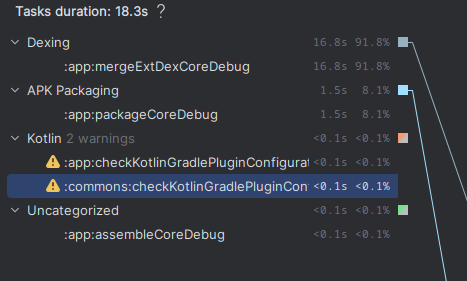
\includegraphics[width=1\linewidth]{Media/img}
    \caption{Application Building}
    \label{fig:Application Building}
\end{figure}


\begin{figure}
    \centering
    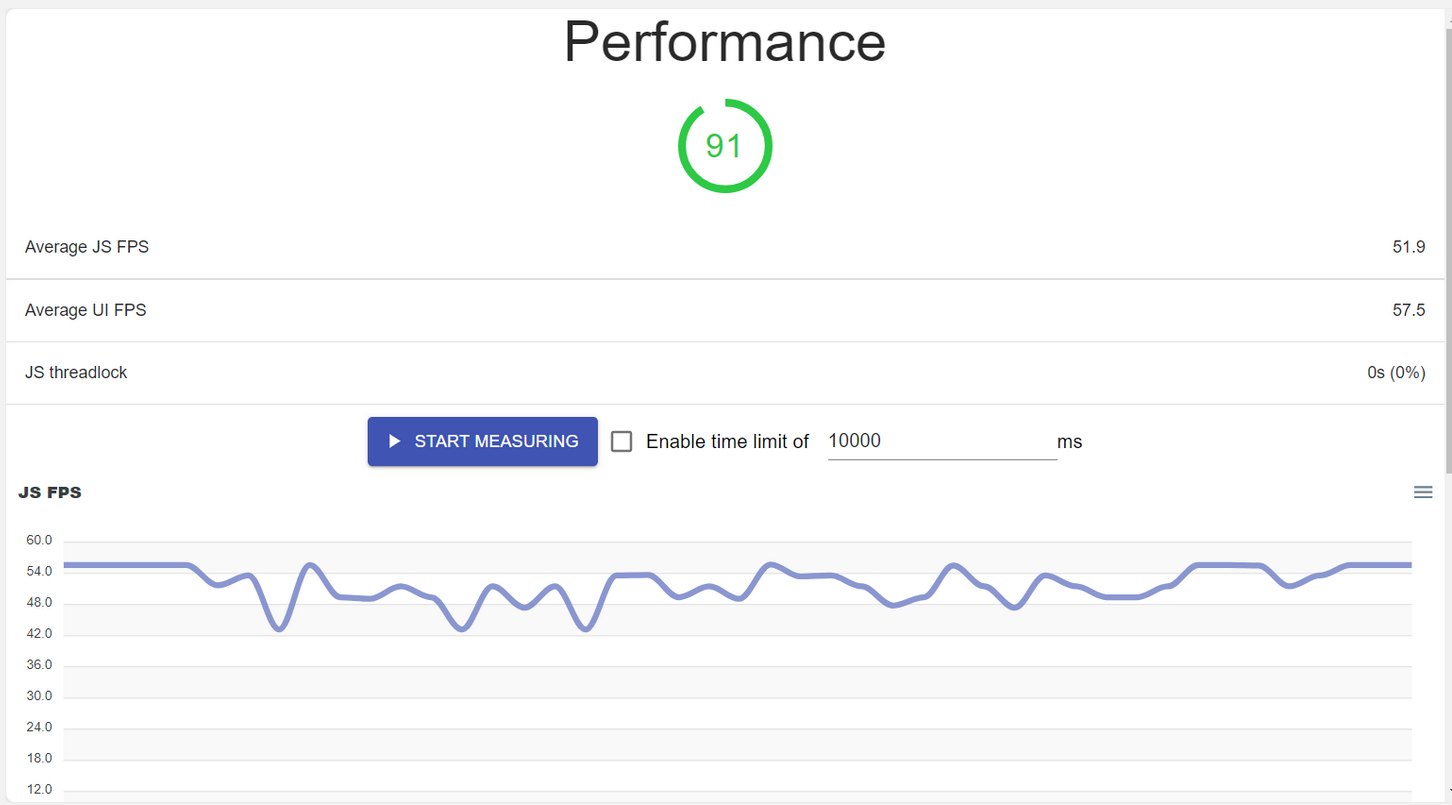
\includegraphics[width=1\linewidth]{Media//Chapter 6/performance}
    \caption{Performance Testing}
    \label{fig: Performance Testing}
\end{figure}

\section{Application Building}\label{sec:app-building}

The process of preparing an application for device deployment includes development, compiling, dexing and  APK packing as shown in the Figure~\ref{fig:Application Building} :

\begin{itemize}
    \item \textbf{Development:} Coding and designing user interface features.
    \item \textbf{Compiling:} Source code conversion into executable bytecode.
    \item \textbf{Dexing:} Android-specific .class to .dex file conversion.
    \item \textbf{APK Packing:} Final app assembly into a downloadable file.
\end{itemize}

\section{Experimental Results}\label{sec:experimental-results}

The experimental results of the testing phase demonstrated the following outcomes:

\begin{enumerate}[label=\roman*.]
    \item \textbf{Functionalities Verified:} All functionalities of the \("\)Call One\("\) app were verified and found to be working as expected.

    \item \textbf{Performance Optimization:} Performance testing revealed that the app performs optimally under various load conditions, ensuring smooth user experience.

\end{enumerate}

After conducting the tests, all the test cases had been passed, the bugs had been fixed, and it's ready to be released.
The flow of testing and fixing the bugs is depicted in the figure.

\section{Screenshots and Photographs}\label{sec:Screenshots od Application Interface}

Visual representations of the tested features, user interface is show in the Figure~\ref{fig:Call One App SignIn Screen},Figure~\ref{fig:Default Dialer Setup and Call Logs Tab},Figure~\ref{fig:Contacts and Call logs Tabs} and Figure~\ref{fig:Profile and Settings}


\begin{figure}
    \centering
    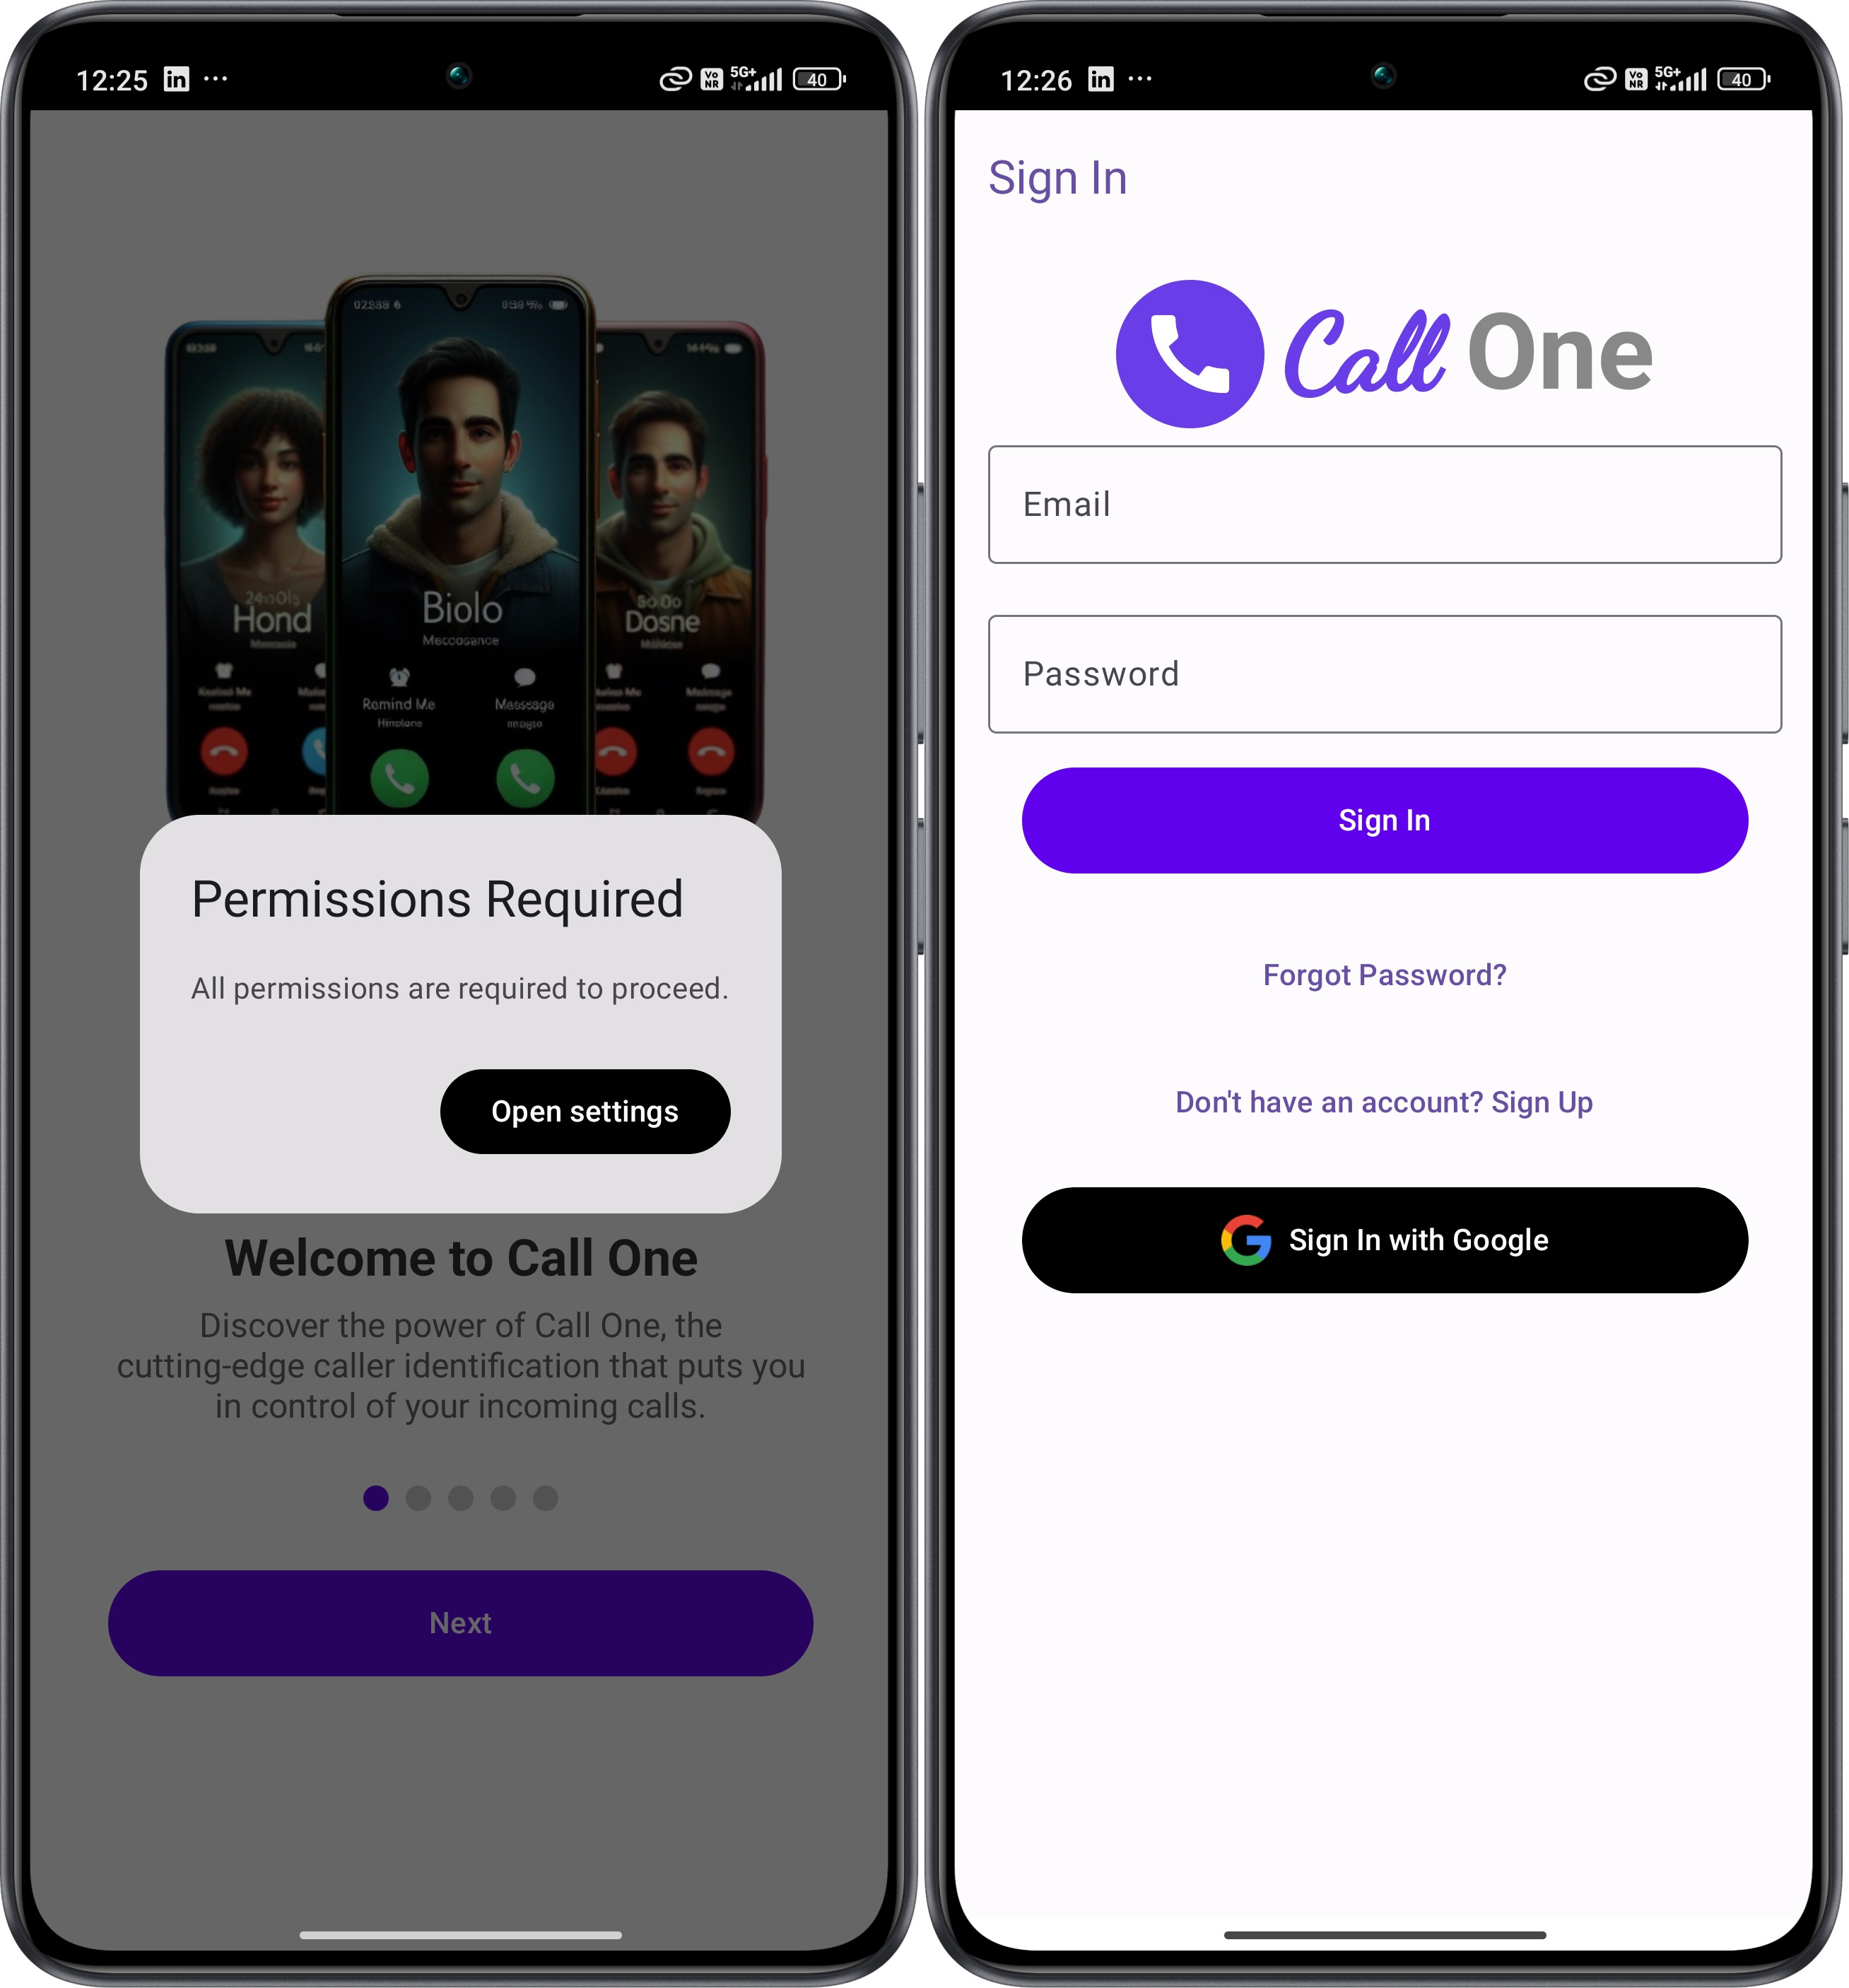
\includegraphics[width=0.5\linewidth]{Media//whatsapp/signin}
    \caption{Call One App SignIn Screen}
    \label{fig:Call One App SignIn Screen}
\end{figure}

\begin{figure}
    \centering
    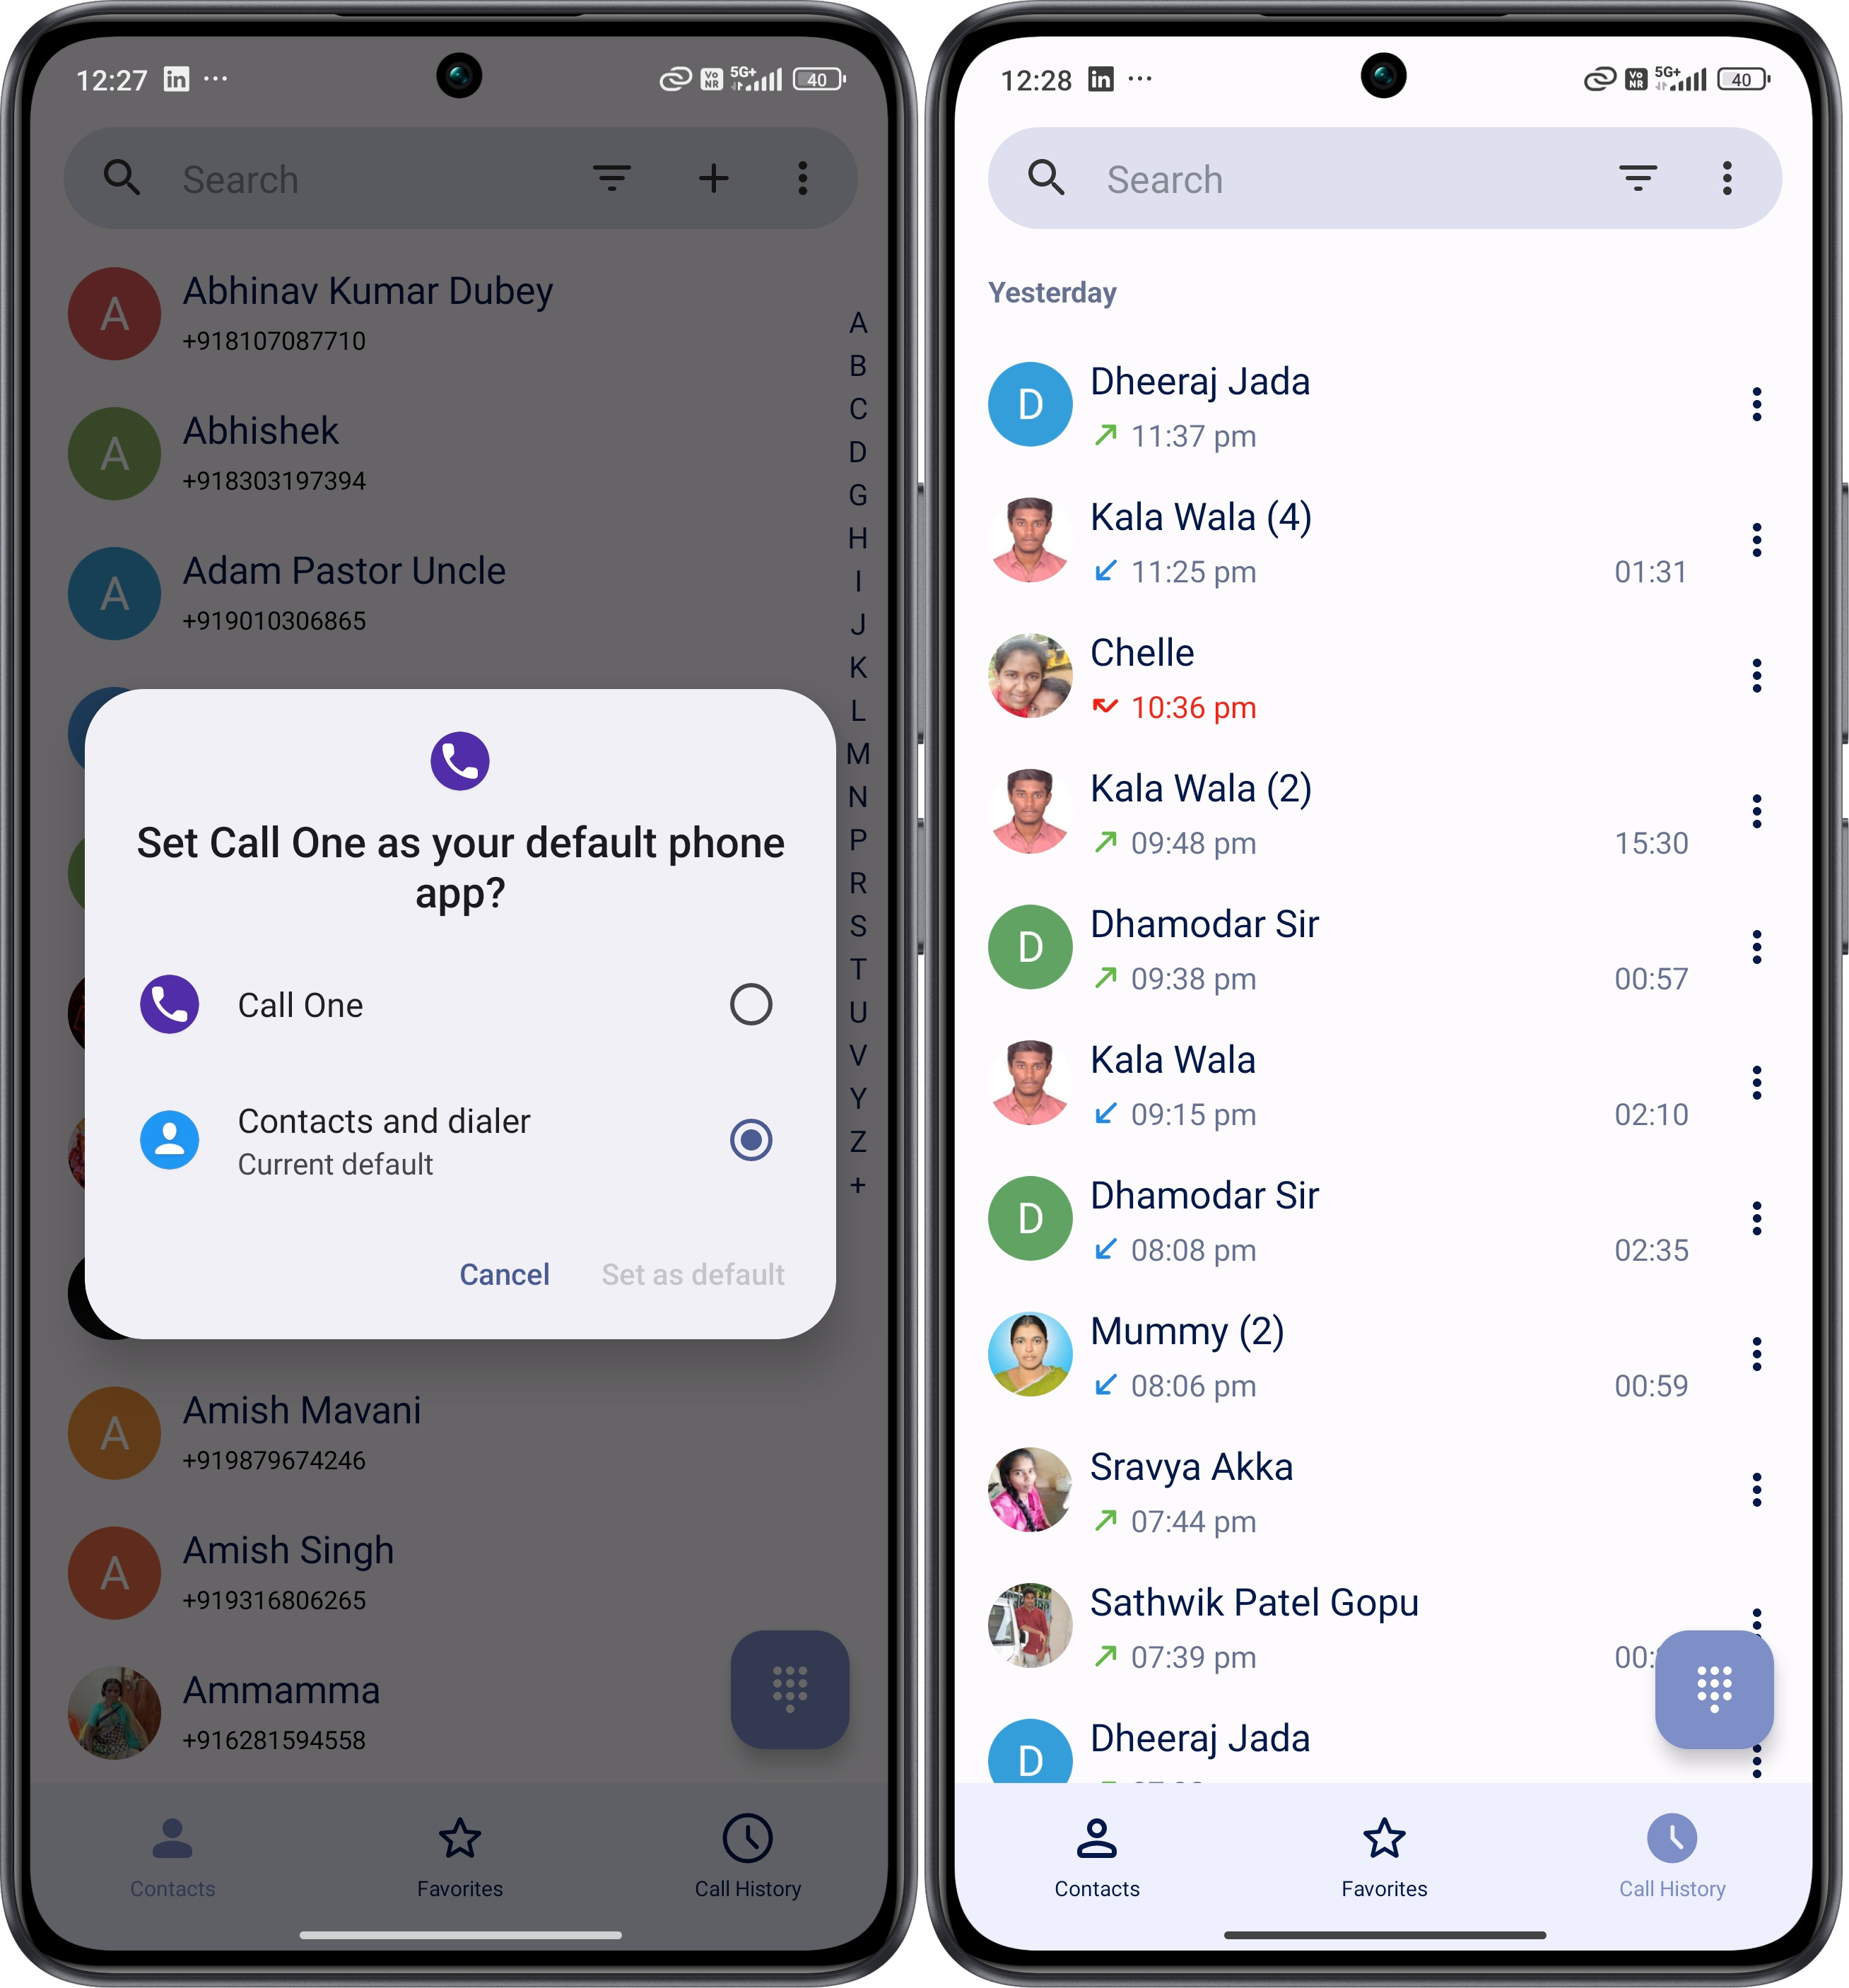
\includegraphics[width=0.5\linewidth]{Media//whatsapp/dd}
    \caption{Default Dialer Setup and Call Logs Tab}
    \label{fig:Default Dialer Setup and Call Logs Tab}
\end{figure}

\begin{figure}
    \centering
    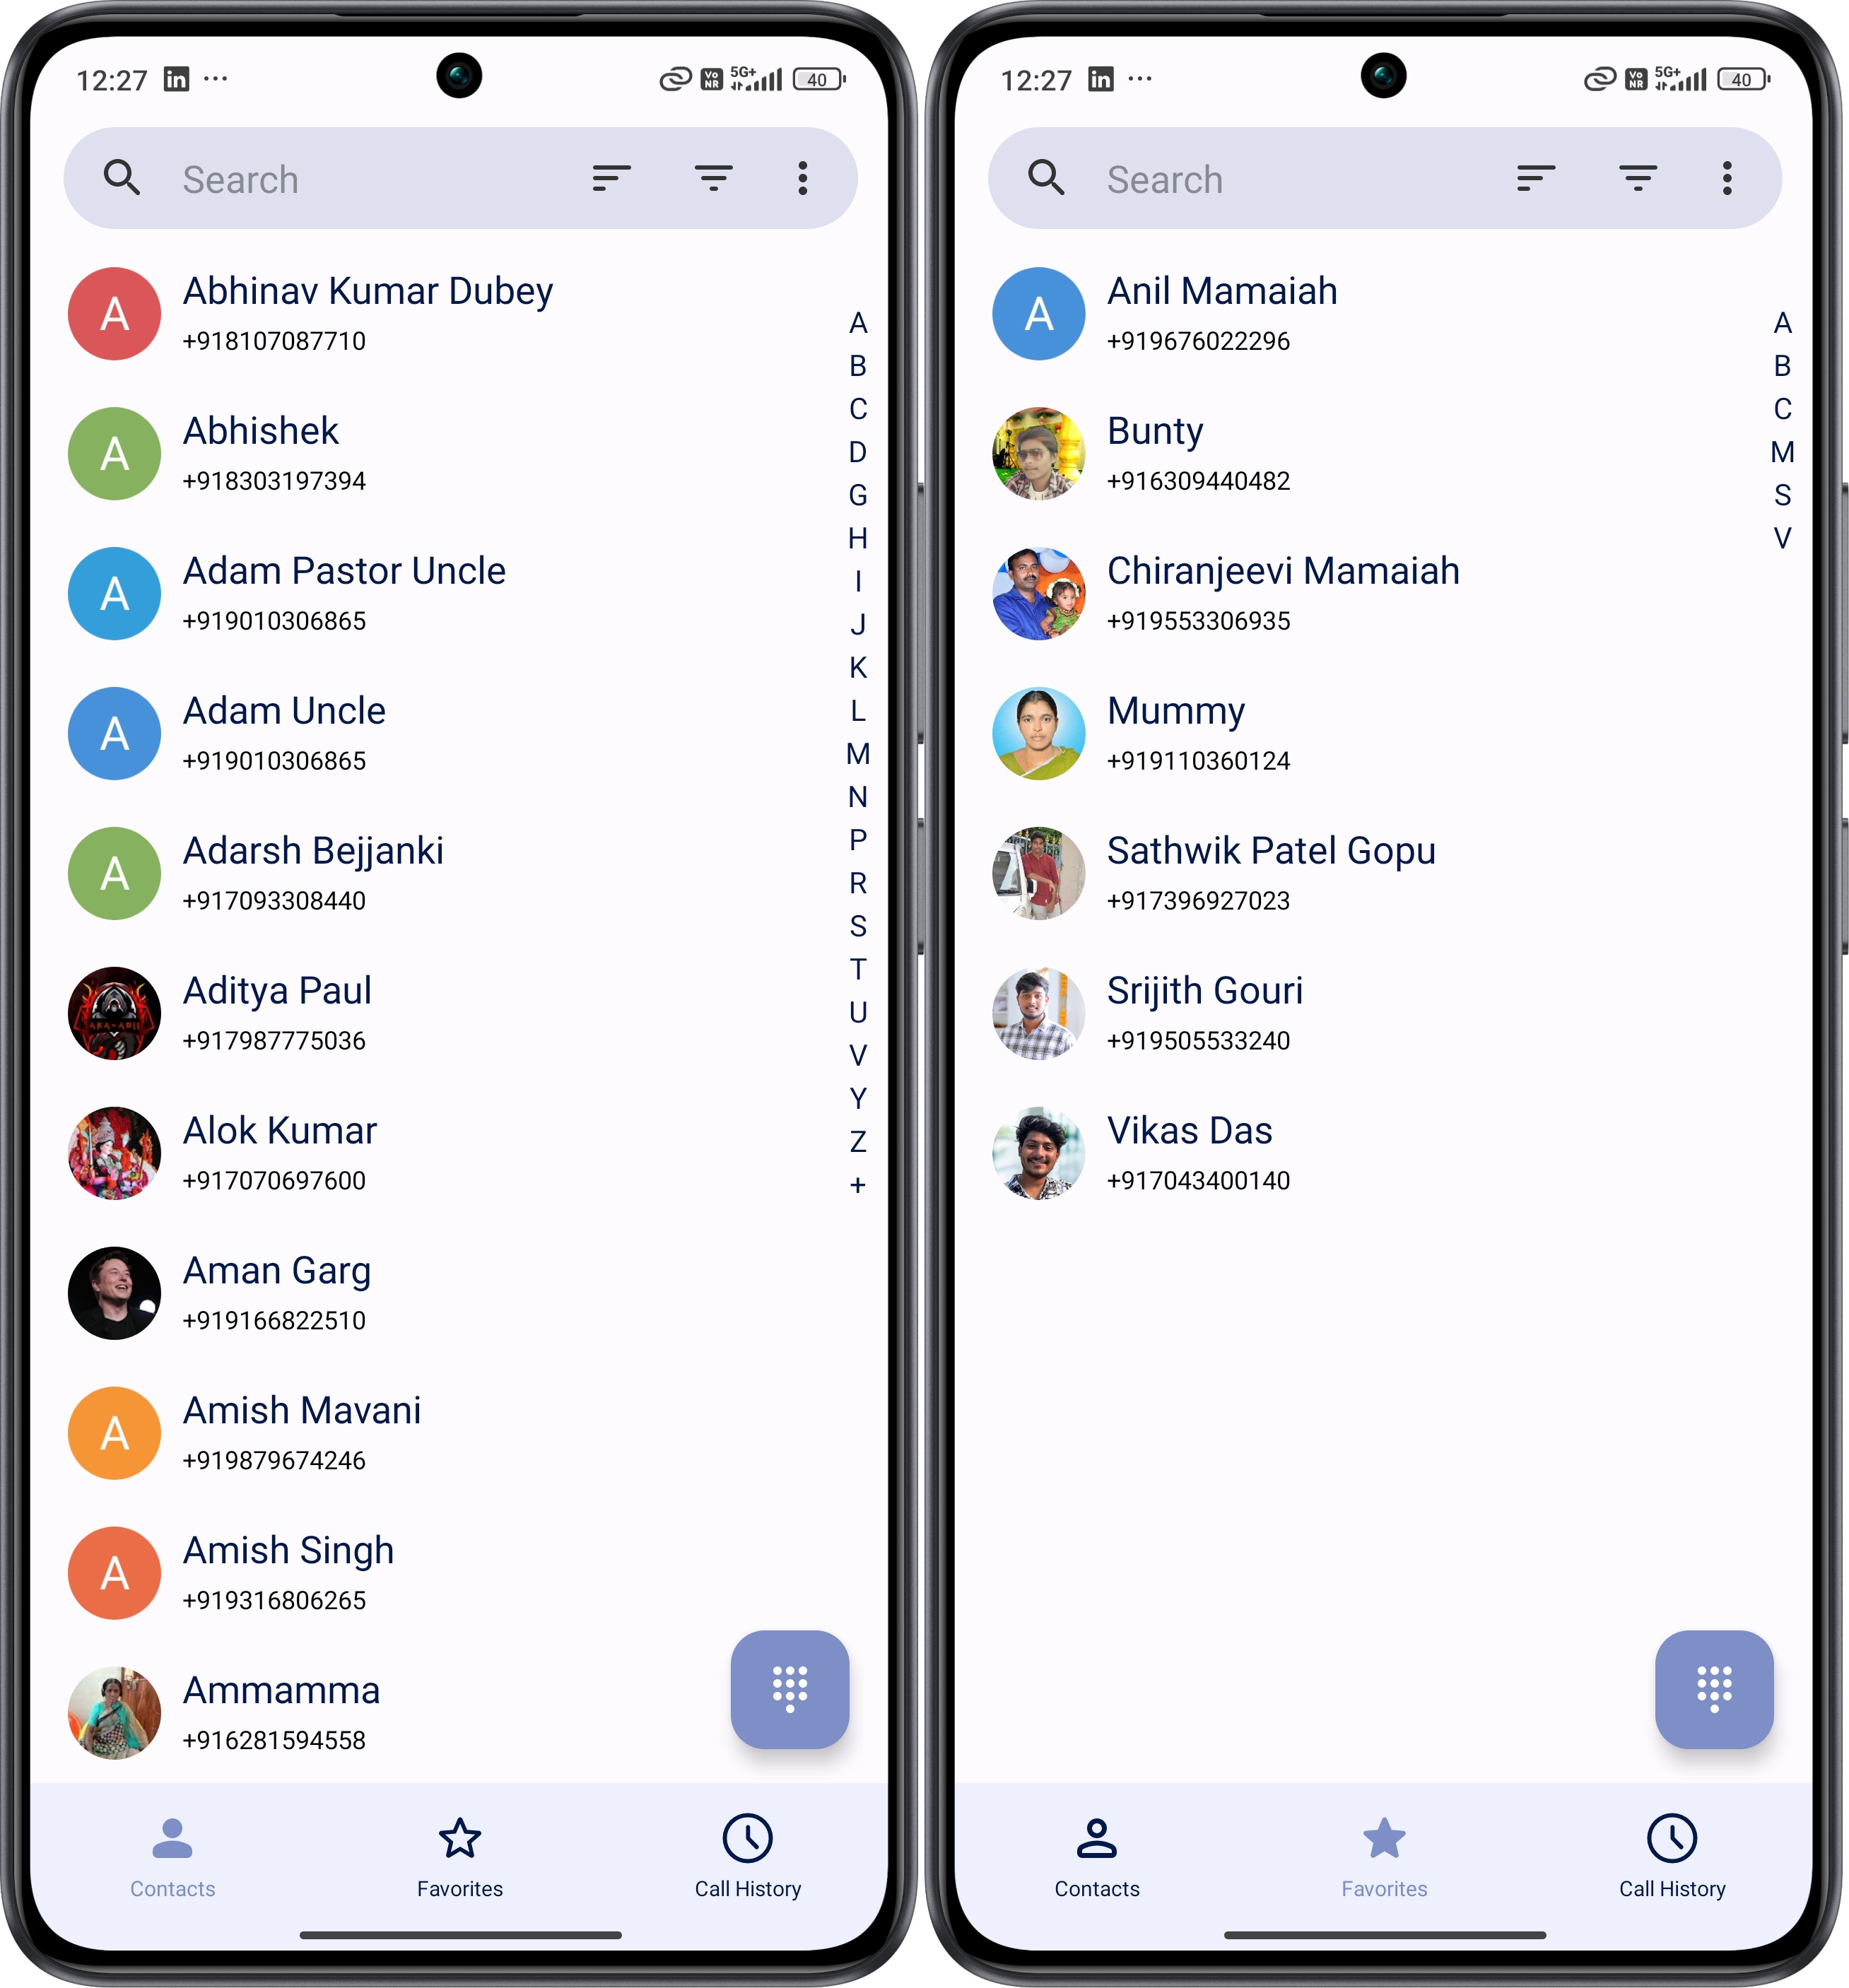
\includegraphics[width=0.5\linewidth]{Media//whatsapp/contactsand}
    \caption{Contacts and Call logs Tabs}
    \label{fig:Contacts and Call logs Tabs}
\end{figure}

\begin{figure}
    \centering
    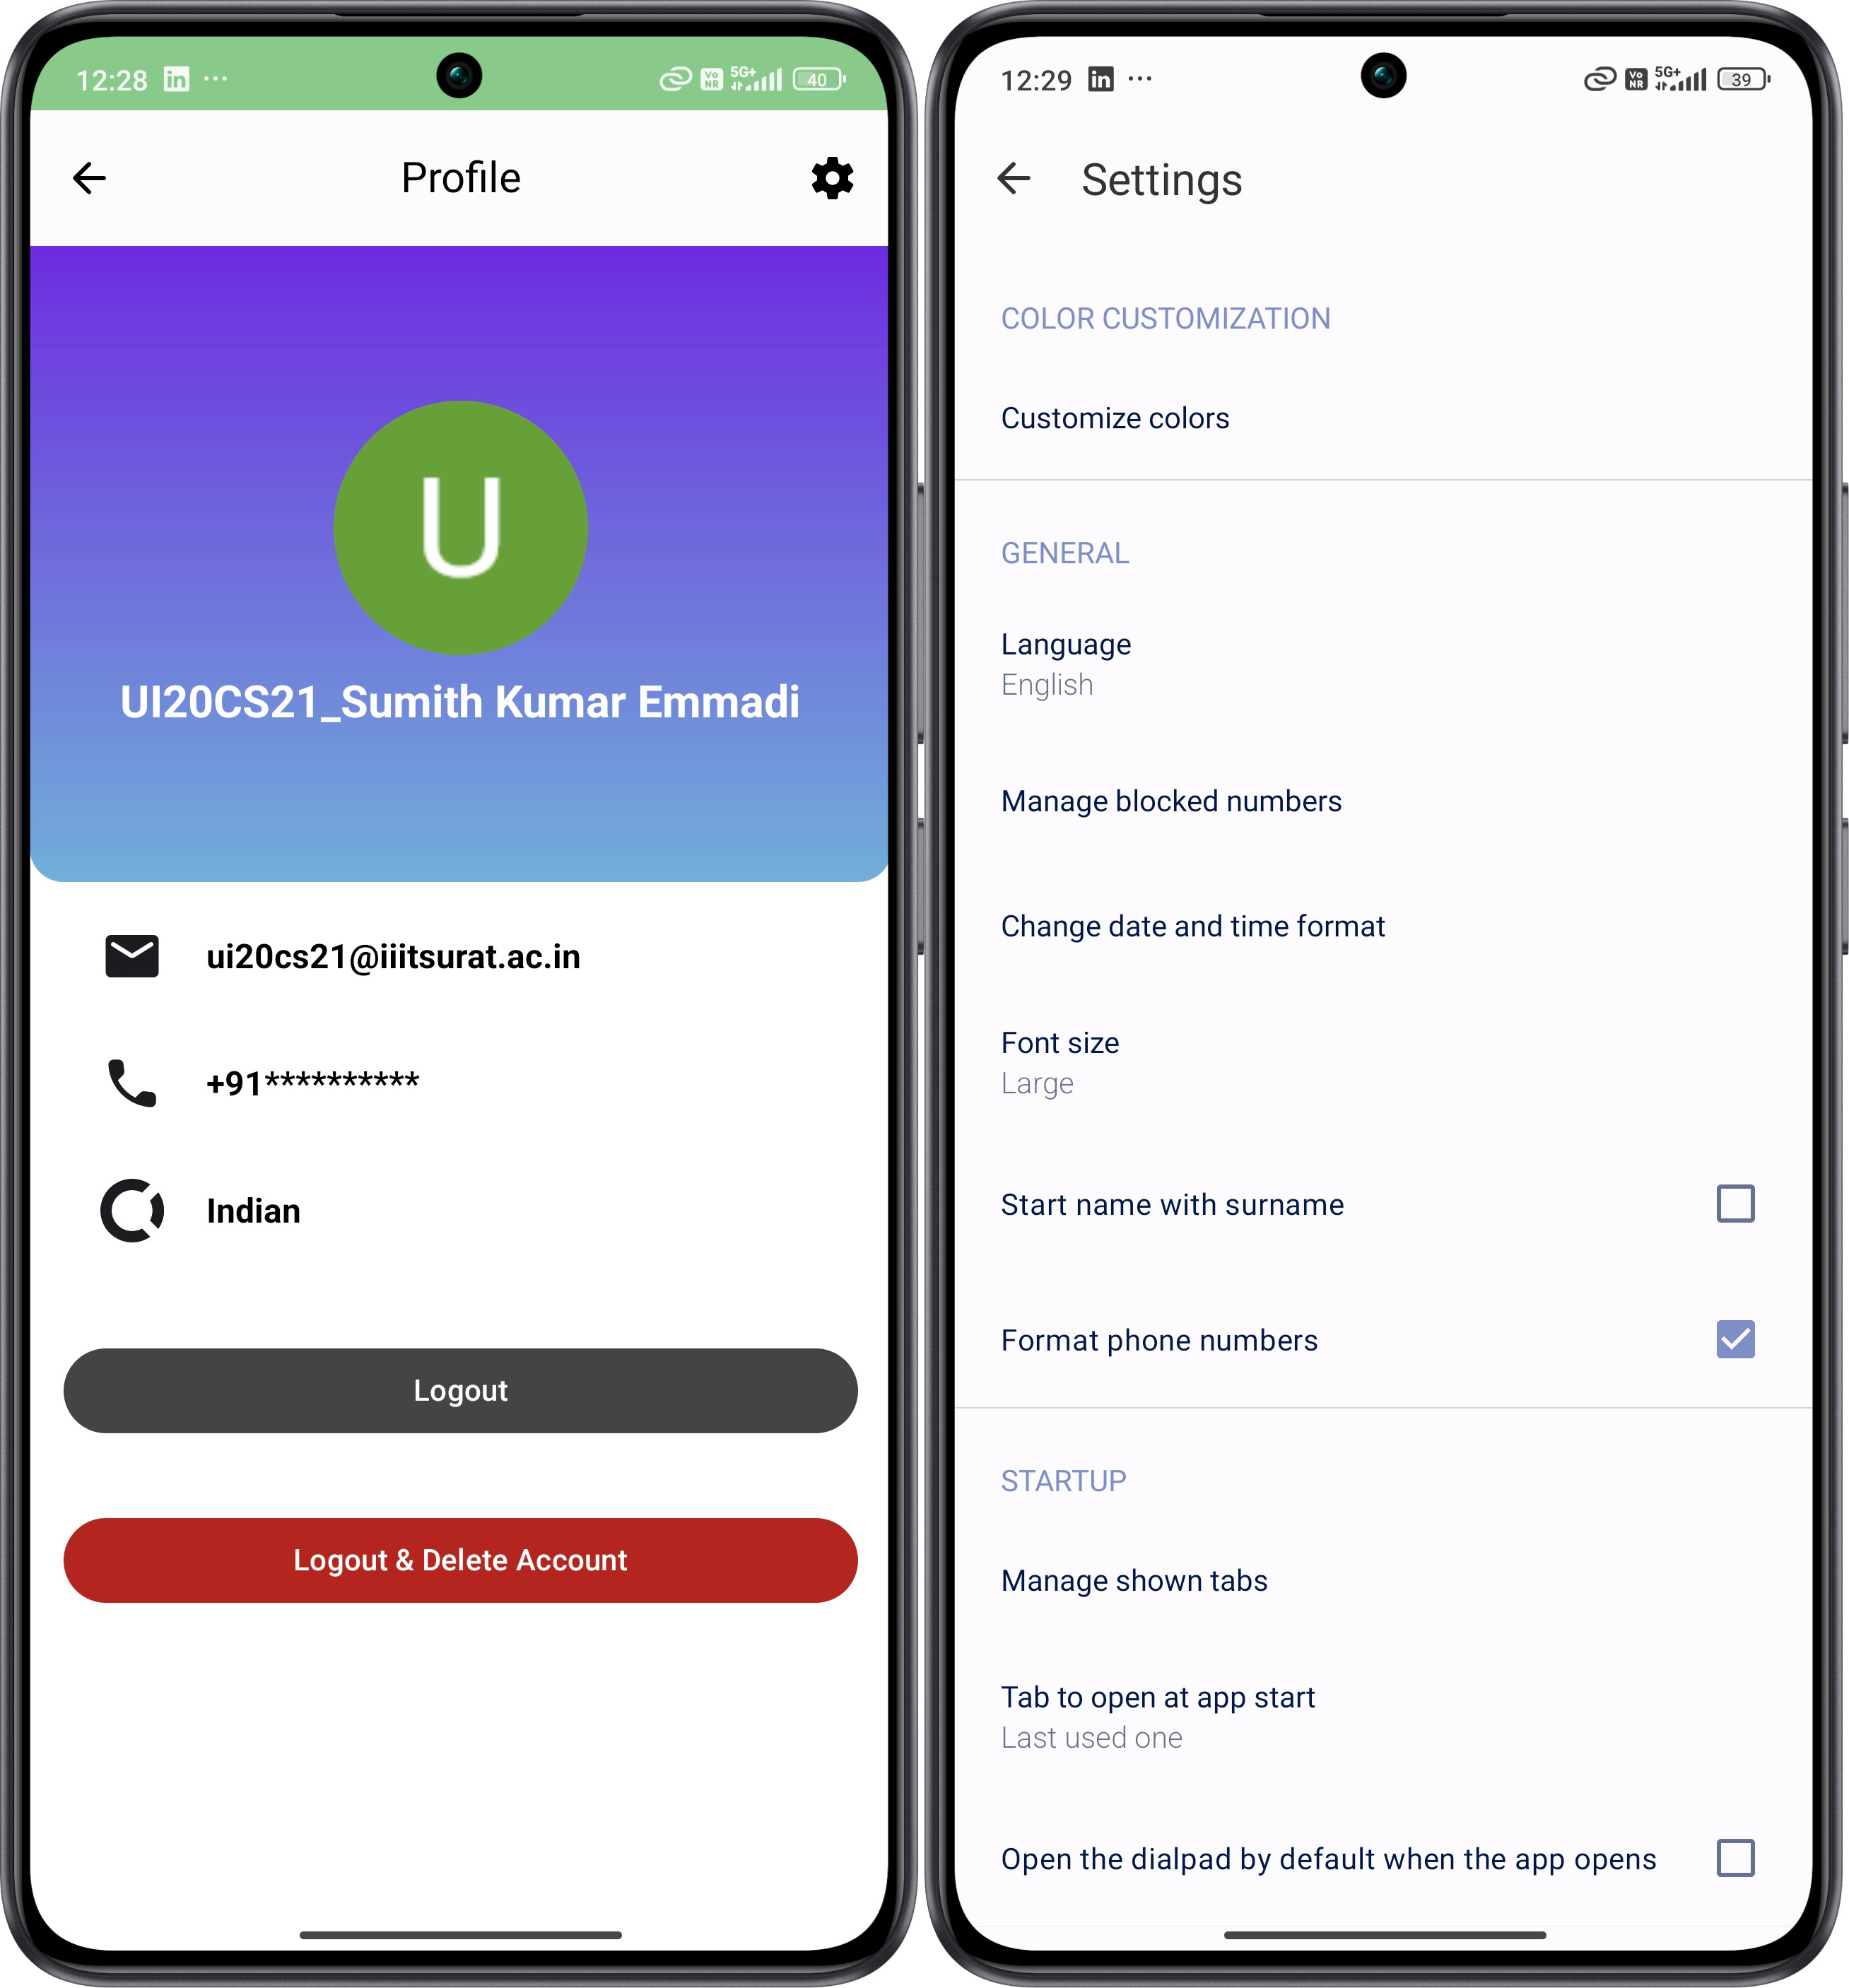
\includegraphics[width=0.5\linewidth]{Media//whatsapp/profile}
    \caption{Profile and Settings}
    \label{fig:Profile and Settings}
\end{figure}

